\documentclass{article}
%packages
% \usepackage{tocloft}
\usepackage{polski}
\usepackage{amsmath}
\usepackage[utf8]{inputenc}
\usepackage{graphicx}
\usepackage{indentfirst}
\usepackage{float}
\usepackage[font=small,labelfont=bf]{caption}
\usepackage[polish]{babel}
\usepackage{hyperref}
\hypersetup{
    colorlinks,
    citecolor=black,
    filecolor=black,
    linkcolor=black,
    urlcolor=black
}
% Variables
\newcommand{\HRule}{\rule{\linewidth}{0.5mm}}
\newcommand{\Prowadzacy}{dr hab. inż. Robert \textsc{Nowicki} prof. PCz}
\newcommand{\Ja}{Piotr \textsc{Filek}\\101311\\I grupa}
\newcommand{\DataLaboratorium}{22 października 2013}
\newcommand{\Uczelnia}{ \textsc{\LARGE Politechnika Częstochowska}\\[1.5cm]}
\newcommand{\Przedmiot}{ \textsc{\Large Podstawy Sieci Komputerowych}\\[1.5cm]}
\newcommand{\TytulLaboratirum}{Laboratorium 3\\Sieć o topologii pierścienia}
\frenchspacing


\begin{document}
\begin{titlepage}
\begin{center}
\Uczelnia
% \textsc{\LARGE Politechnika Częstochowska}\\[1.5cm]
\Przedmiot% \textsc{\Large Final year project}\\[0.5cm]
\HRule\\[0.4cm]
{ \huge \bfseries \TytulLaboratirum \\[0.4cm] }
% { \huge \bfseries Large brewing techniques \\[0.4cm]}
\HRule\\[1.5cm]

% Author and supervisor
\begin{minipage}[t]{0.4\textwidth}
\begin{flushleft}\large
\emph{Autor:}\\
\Ja
\end{flushleft}
\end{minipage}
\begin{minipage}[t]{0.5\textwidth}
\begin{flushright} \large
\emph{Prowadzący:} \\
\Prowadzacy
\end{flushright}
\end{minipage}

\vfill

% Bottom of the page
{\large \DataLaboratorium}

\end{center}
\end{titlepage}
\newpage
\section{Cel laboratorium}

Celem laboratorium było zpoznanie się z działaniem sieci o topologii pierścienia, na przykładzie technologii Token Ring. Wykorzystanie wyników uzyskanych w poprzednich ćwiczeniach pozwoliło również na porównanie działania tego typu sieci z sieciami o medium współdzielonym (logiczna magistrala) oraz przełączanym. Cel ten został uzyskany poprzez porównanie następujących przypadków:
\begin{itemize}
\item sieć o topologii pierścienia o architekturze równorzędnej (ang. \textit{peer to peer}),
\item sieć o topologii pierścienia o architekturze klient-serwer.

\end{itemize}
Zbadany został także wpływ stacji oraz natężenia ruchu w sieci.
\section{Wyniki}


\begin{figure}[H]
  \centering
  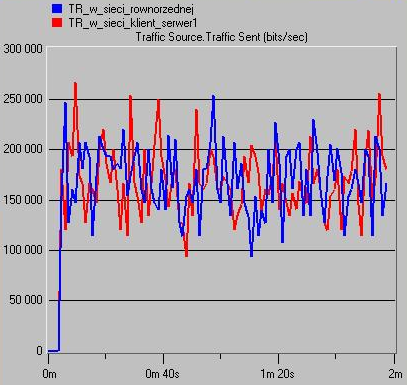
\includegraphics[width=0.65\textwidth]{screens/2_sent.png}
 \caption{Wykres przedstawiający ilość bitów/sec wysłanych dla sieci z 2 stacjami roboczymi}
 \label{fig:2s}
\end{figure}


\begin{figure}[H]
  \centering
  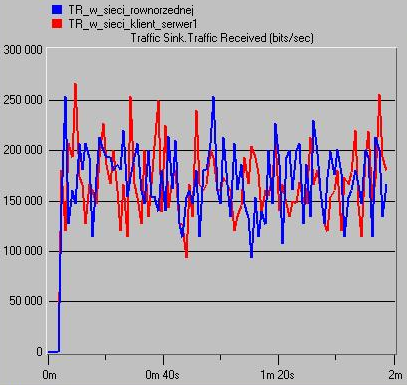
\includegraphics[width=0.65\textwidth]{screens/2_recv.png}
 \caption{Wykres przedstawiający ilość bitów/sec odebranych dla sieci z 2 stacjami roboczymi}
 \label{fig:2r}
\end{figure}

\begin{figure}[H]
  \centering
  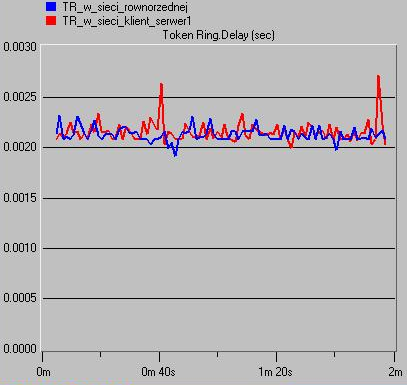
\includegraphics[width=0.65\textwidth]{screens/2_delay.png}
 \caption{Wykres przedstawiający opóźnienia w sieci z 2 stacjami roboczymi}
 \label{fig:2d}
\end{figure}

\begin{figure}[H]
  \centering
  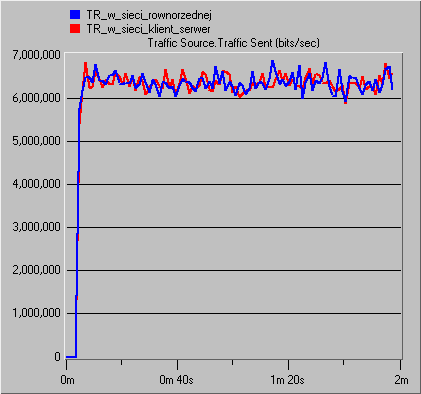
\includegraphics[width=0.65\textwidth]{screens/4_sent.png}
 \caption{Wykres przedstawiający ilość bitów/sec wysłanych dla sieci z 4 stacjami roboczymi}
 \label{fig:4s}
\end{figure}


\begin{figure}[H]
  \centering
  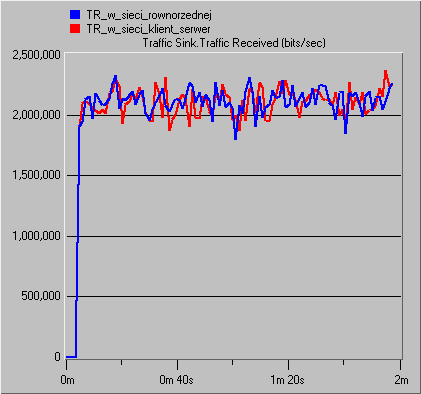
\includegraphics[width=0.65\textwidth]{screens/4_recv.png}
 \caption{Wykres przedstawiający ilość bitów/sec odebranych dla sieci z 4 stacjami roboczymi}
 \label{fig:4r}
\end{figure}

\begin{figure}[H]
  \centering
  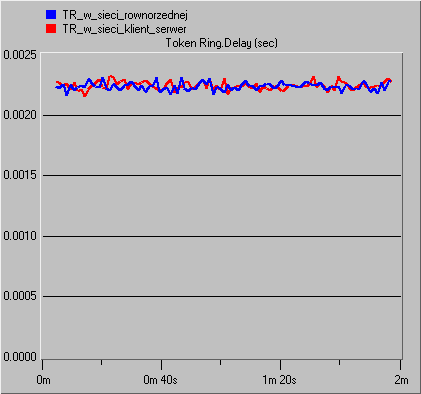
\includegraphics[width=0.65\textwidth]{screens/4_delay.png}
 \caption{Wykres przedstawiający opóźnienia w sieci z 4 stacjami roboczymi}
 \label{fig:4d}
\end{figure}


\begin{figure}[H]
  \centering
  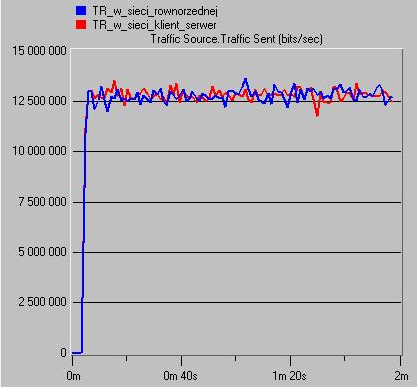
\includegraphics[width=0.65\textwidth]{screens/8_sent.png}
 \caption{Wykres przedstawiający ilość bitów/sec wysłanych dla sieci z 8 stacjami roboczymi}
 \label{fig:8s}
\end{figure}


\begin{figure}[H]
  \centering
  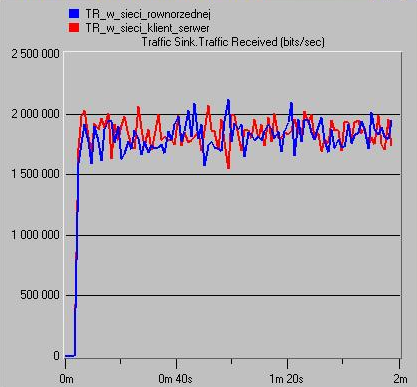
\includegraphics[width=0.65\textwidth]{screens/8_recv.png}
 \caption{Wykres przedstawiający ilość bitów/sec odebranych dla sieci z 8 stacjami roboczymi}
 \label{fig:8r}
\end{figure}

\begin{figure}[H]
  \centering
  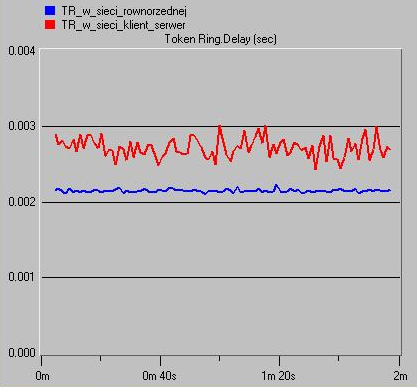
\includegraphics[width=0.65\textwidth]{screens/8_delay.png}
 \caption{Wykres przedstawiający opóźnienia w sieci z 8 stacjami roboczymi}
 \label{fig:8d}
\end{figure}

\begin{figure}[H]
  \centering
  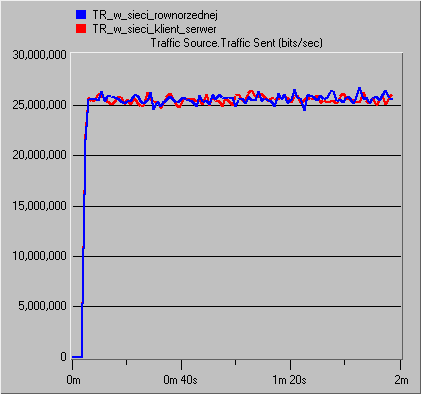
\includegraphics[width=0.65\textwidth]{screens/16_sent.png}
 \caption{Wykres przedstawiający ilość bitów/sec wysłanych dla sieci z 16 stacjami roboczymi}
 \label{fig:16s}
\end{figure}


\begin{figure}[H]
  \centering
  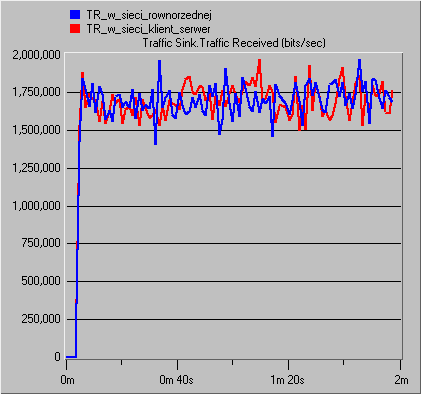
\includegraphics[width=0.65\textwidth]{screens/16_recv.png}
 \caption{Wykres przedstawiający ilość bitów/sec odebranych dla sieci z 16 stacjami roboczymi}
 \label{fig:16r}
\end{figure}

\begin{figure}[H]
  \centering
  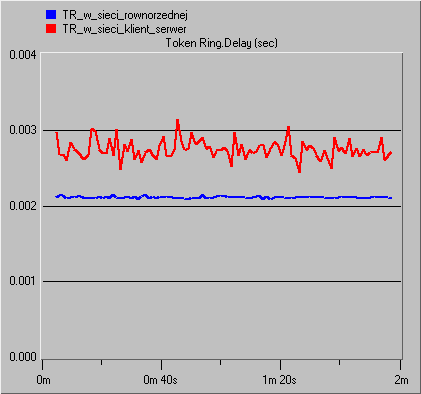
\includegraphics[width=0.65\textwidth]{screens/16_delay.png}
 \caption{Wykres przedstawiający opóźnienia w sieci z 16 stacjami roboczymi}
 \label{fig:16d}
\end{figure}

\begin{figure}[H]
  \centering
  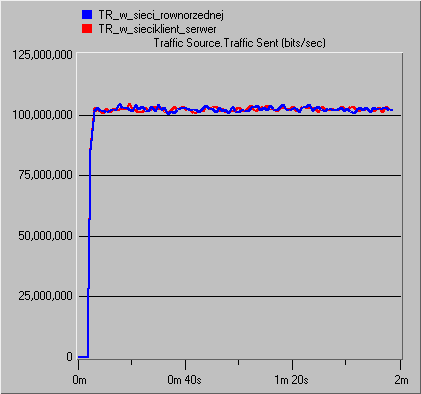
\includegraphics[width=0.65\textwidth]{screens/64_sent.png}
 \caption{Wykres przedstawiający ilość bitów/sec wysłanych dla sieci z 64 stacjami roboczymi}
 \label{fig:64s}
\end{figure}


\begin{figure}[H]
  \centering
  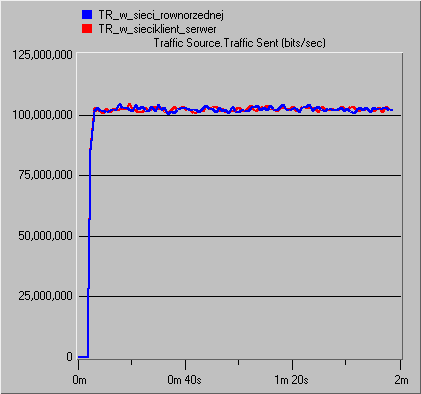
\includegraphics[width=0.65\textwidth]{screens/64_recv.png}
 \caption{Wykres przedstawiający ilość bitów/sec odebranych dla sieci z 64 stacjami roboczymi}
 \label{fig:64r}
\end{figure}

\begin{figure}[H]
  \centering
  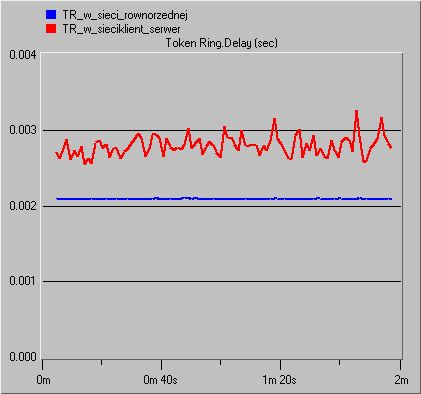
\includegraphics[width=0.65\textwidth]{screens/64_delay.png}
 \caption{Wykres przedstawiający opóźnienia w sieci z 64 stacjami roboczymi}
 \label{fig:64d}
\end{figure}

\begin{figure}[H]
  \centering
  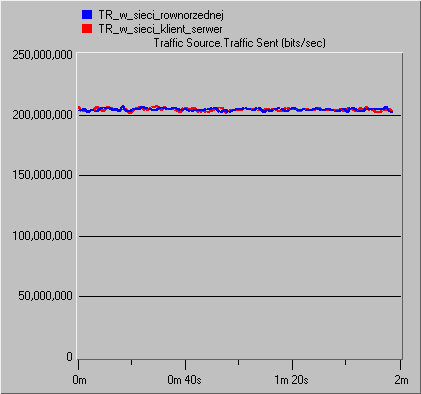
\includegraphics[width=0.65\textwidth]{screens/128_sent.png}
 \caption{Wykres przedstawiający ilość bitów/sec wysłanych dla sieci z 128 stacjami roboczymi}
 \label{fig:128s}
\end{figure}


\begin{figure}[H]
  \centering
  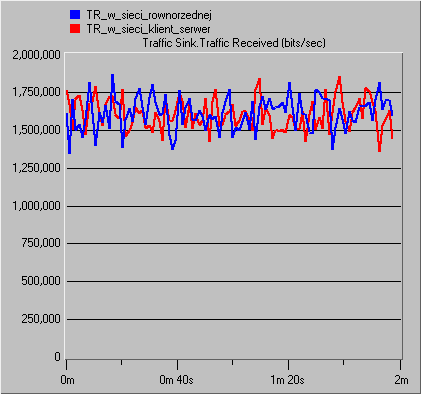
\includegraphics[width=0.65\textwidth]{screens/128_recv.png}
 \caption{Wykres przedstawiający ilość bitów/sec odebranych dla sieci z 128 stacjami roboczymi}
 \label{fig:128r}
\end{figure}

\begin{figure}[H]
  \centering
  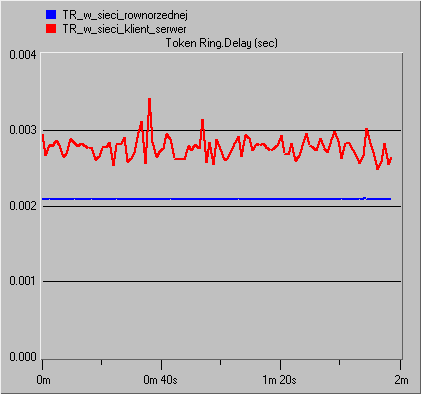
\includegraphics[width=0.65\textwidth]{screens/128_delay.png}
 \caption{Wykres przedstawiający opóźnienia w sieci z 128 stacjami roboczymi}
 \label{fig:128d}
\end{figure}

\section{Wnioski}
W pierścieniu sieci \emph{Token Ring} krąży mała ramka zwana \emph{żetonem} (ang. \textit{token}). Stacja sieciowa uzyskuje prawo do transmisji informacji \emph{tylko} wtedy, gdy posiada token. Jeśli więc dowolna stacja sieciowa przejmuje token, ale w tym momencie nie zamierza transmitować, to przesyła żeton do następnej w kolejności stacji sieciowej. Każda stacja może przetrzymywać token tylko przez określony czas.

Opóźnienia w sieci \emph{Token Ring} są praktycznie zerowe i nie zwiększają się wraz ze wzrostem ilości stacji czy też obciążeniem w sieci, podobnie jakt to jest w sieci typu \emph{Ethernet} opartej na przełączniku. Kolizje występują jedynie w sieci \emph{Ethernet} opartej na \emph{koncentratorze}.

\emph{Token Ring} został wyparty przez switched \emph{Ethernet} który szybciej się rozwijał, obsługiwał większą ilość urządzeń oraz fakt, że budowa sieci Ethernet jest łatwiejsza w realizacji i nie wymaga dogłębnego zrozumienia protokołu, jak to jest w przypadku \emph{Token Ring}.

Sieć o topologii pierścienia, w przeciwieństwie do sieci o topologii gwiazdy, nie wymaga żadnego medium transmitującego. Powoduje to zmniejszenie kosztów, jednakże może to zwiększyć awaryjność sieci - awaria pojedyńczego przewodu lub komputera powoduje przerwanie pracy całej sieci. Podpięcie nowej stacji roboczej do sieci, czy też lokalizacja uszkodzenia jest dużo trudniejsza niż w sieci o topologii gwiazdy.

\end{document}